%!TeX root=../tese.tex
%("dica" para o editor de texto: este arquivo é parte de um documento maior)

% Conteúdo da subseção sobre Viagens
% Este arquivo é importado em 02-implementacao.tex

Durante os seis meses do piloto BikeSP, foram registradas mais de 29.000 viagens pelo aplicativo Android dos participantes, totalizando mais de 150.000 km pedalados. Este volume de dados demandou interface robusta para visualização, busca e análise pela equipe de suporte e pesquisadores. A tela de viagens tornou-se ferramenta essencial para diagnóstico de problemas reportados por usuários (``minha viagem não apareceu'', ``valor creditado está incorreto''), validação de contestações, e análises exploratórias para publicações científicas.

A tabela de viagens apresenta oito colunas principais: ID da viagem (identificador único), ID do usuário, data da viagem, deslocamento em metros, IDs de origem e destino (referenciando localizações cadastradas), status (aprovada/reprovada), e remuneração calculada em reais. O sistema consulta dados de viagens vinculando informações de pessoas e localizações de origem e destino, utilizando técnicas de paginação eficiente para responsividade. Ordenação padrão por ID decrescente exibe viagens mais recentes primeiro, padrão adequado para monitoramento operacional diário.

O campo de busca permite filtrar viagens por ID de usuário específico (busca exata). Esta funcionalidade atende cenário operacional frequente: participante relata problema com viagem; administrador identifica ID do usuário na tela de participantes; busca todas viagens daquele usuário; localiza a viagem em questão (geralmente reconhecível por data/horário ou trajeto).

 \begin{figure}[H]
   \centering
   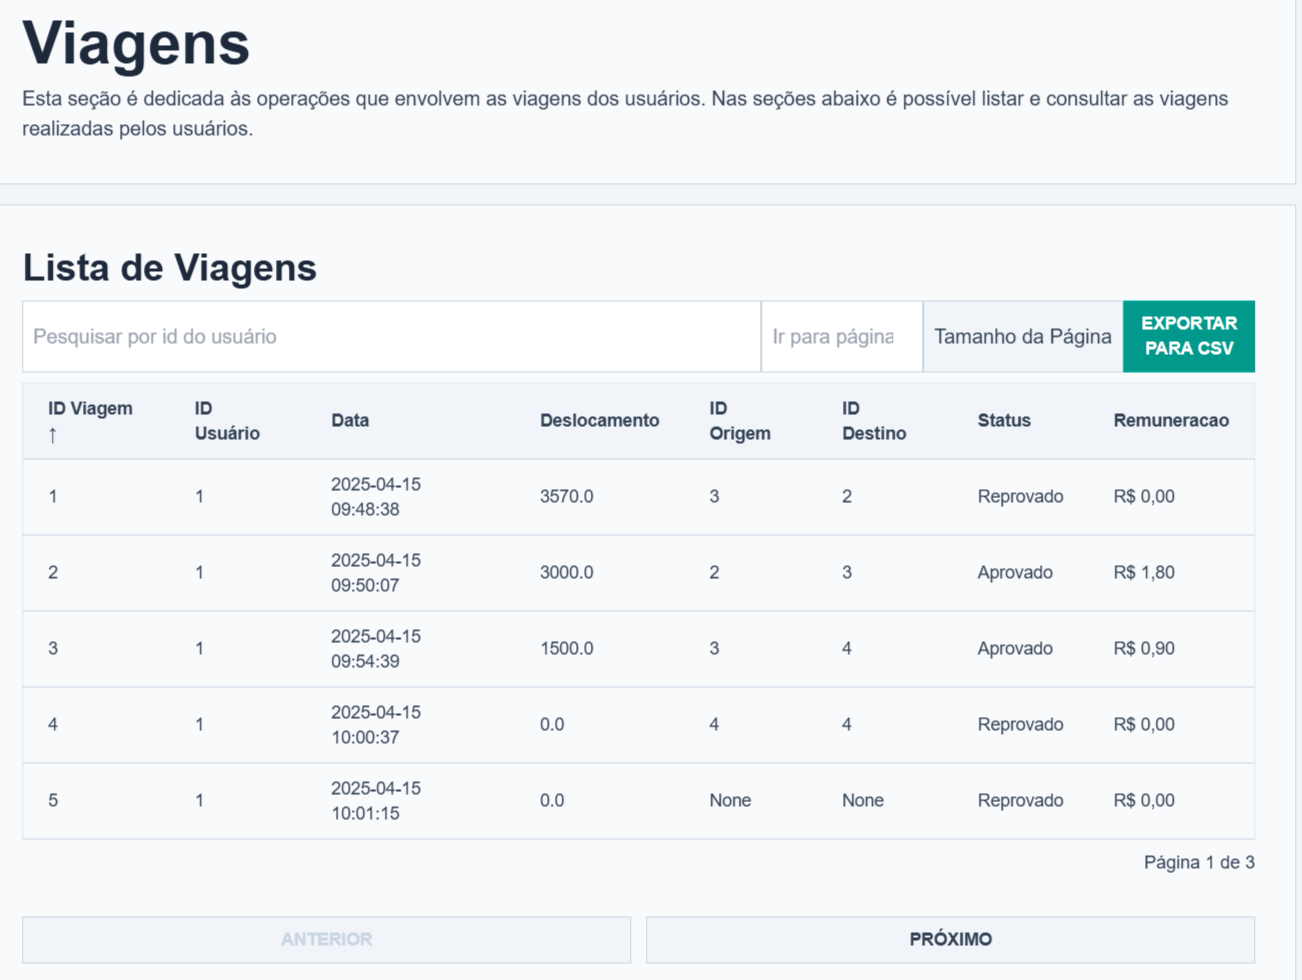
\includegraphics[width=0.95\textwidth]{figuras/viagens_listar.png}
   \caption{Interface de listagem de viagens com funcionalidades de busca, ordenação e paginação.}
   \label{fig:viagens_listar}
 \end{figure}

Ao clicar em qualquer linha da tabela, a interface renderiza mapa interativo (biblioteca Leaflet.js com tiles OpenStreetMap) exibindo trajeto completo da viagem abaixo da tabela. O mapa plota marcadores para cada ponto GPS coletado pelo aplicativo durante a viagem, conectados por linha azul na ordem temporal. Popups nos marcadores exibem timestamp de cada ponto. Zoom automático enquadra toda rota, e controles padrão (zoom, pan, scroll) permitem inspeção detalhada. Esta funcionalidade revelou-se crítica para validação de viagens contestadas: administradores visualizavam se trajeto realmente conectava origem e destino declarados, se passava por vias adequadas para ciclismo, e se não apresentava anomalias (ex: teletransportes indicando GPS incorreto).

\begin{figure}[H]
    \centering
    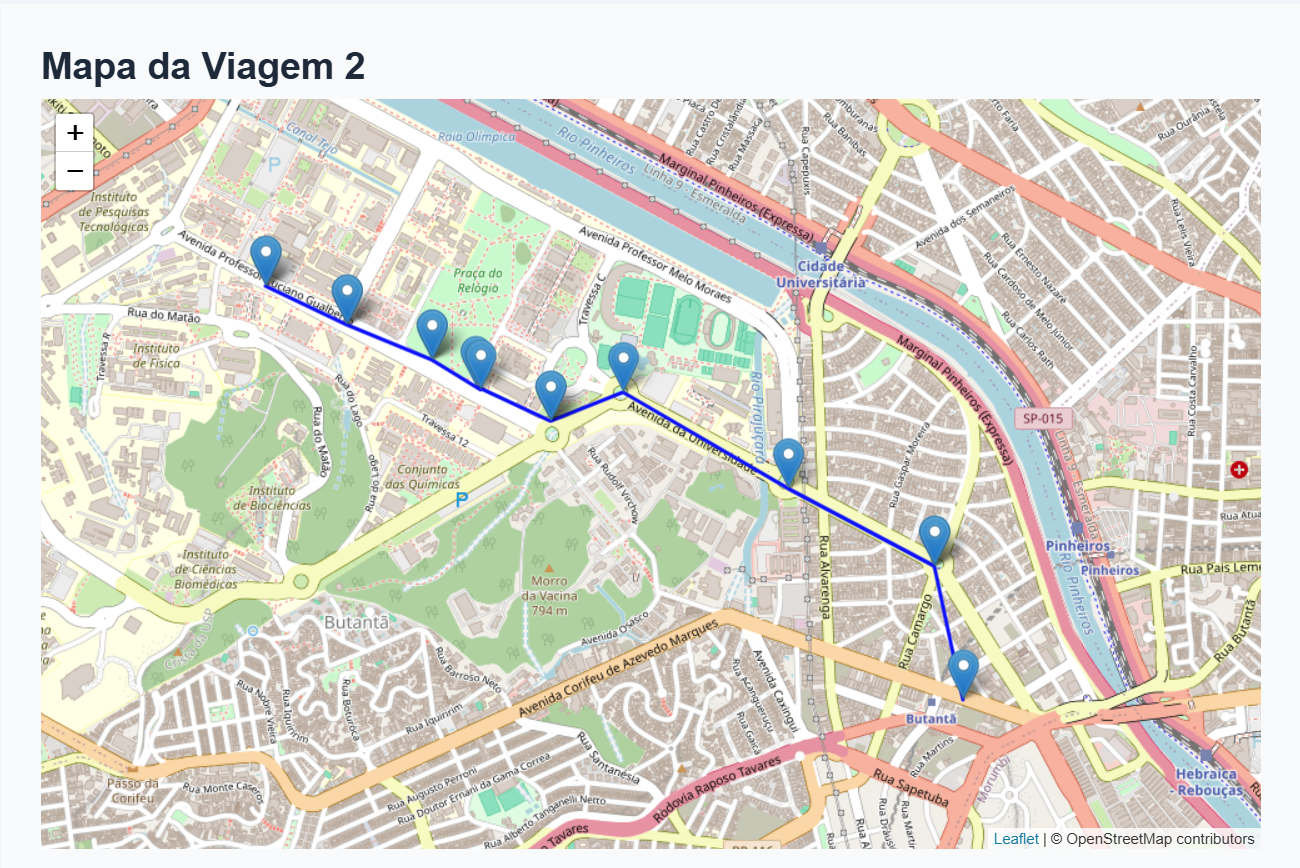
\includegraphics[width=0.95\textwidth]{figuras/mapa_contestacao.PNG}
    \caption{Visualização de trajeto de viagem fictícia com origem no IME e destino na estação Butantã no mapa interativo com marcadores de pontos GPS.}
    \label{fig:mapa_contestacao}
  \end{figure}

O botão de exportação gera arquivo CSV contendo todas as informações exibidas (respeitando filtros de busca ativos) para análise em ferramentas externas. O formato inclui cabeçalho descritivo e delimitador ponto-e-vírgula. Durante piloto, esta funcionalidade foi utilizada semanalmente por economistas do projeto para análises estatísticas: modelos de regressão investigando impacto das coortes no número de viagens, análises de série temporal identificando padrões de uso ao longo da semana, e visualizações geoespaciais em GIS identificando origens/destinos mais frequentes. A possibilidade de exportar dados filtrados (ex: apenas viagens de determinado usuário ou período) reduziu necessidade de consultas diretas ao banco de dados para análises.

A ordenação por diferentes colunas viabiliza análises rápidas: ordenar por deslocamento descendente identifica viagens mais longas (útil para identificar outliers ou comportamento atípico); ordenar por data permite inspeção cronológica (verificar se sistema registrou viagens durante manutenções); ordenar por status agrupa aprovadas vs. reprovadas (calcular taxa de aprovação manual); ordenar por remuneração identifica viagens de maior valor. Durante análise dos resultados do piloto, observou-se que 9 das 10 viagens mais longas (identificadas via ordenação por deslocamento) ocorreram em finais de semana sem remuneração, evidência importante de retenção intrínseca do hábito de pedalar para além do incentivo financeiro.

A configuração padrão de 10 viagens por página balanceia densidade de informação e tempo de carregamento. Com 29.000+ registros, carregar todas viagens simultaneamente seria inviável; paginação server-side (LIMIT/OFFSET no PostgreSQL) mantém responsividade independente do volume total. Indicador ``Página X de Y'' fornece senso de escala, reforçando necessidade de busca e ordenação para localizar informação relevante. Opções de 5, 15 ou 20 itens por página atendem diferentes casos de uso: densidade baixa para inspeção cuidadosa com múltiplos mapas abertos; densidade alta para varredura rápida de padrões.

\textit{Cenário 1: Diagnóstico de viagem não creditada} --- participante relata viagem realizada ontem não apareceu no extrato; administrador busca por ID do usuário, filtra viagens recentes (ordenação por data), identifica viagem com status ``reprovada''; visualiza mapa, constata que trajeto passou por localizações não cadastradas; orienta participante a atualizar endereços. \textit{Cenário 2: Validação de contestação} --- usuário contesta rejeição de viagem; administrador abre viagem contestada, visualiza mapa, confirma que trajeto conecta origem e destino cadastrados; aprova contestação, gerando remuneração retroativa.


